\documentclass[a4paper]{hitec}
\settextfraction{0.95}      % reduce left margin

\usepackage{styles/main}
\usepackage{styles/custom}
\usepackage[T1]{fontenc}
\usepackage[utf8]{inputenc}


\author{Michael Hofer}
\company{HTBLA Weiz}

% ----- Informationen über die Diplomarbeit -----

\htltitle{Projektname}
\AbgabeTermin{28.03.2023}

\DeckblattBild{images/emily.jpg}

\Diplomand{Diplomand 1}{5AHET}
\Diplomand{Diplomand 2}{5BHET}
\Diplomand{Diplomand 3}{5AHMBT}
\Diplomand{Diplomand 4}{5AHMBU}
\Diplomand{Diplomand X}{5AHWIM}

\Betreuer{Betreuer 1}
\Betreuer{Betreuer X}

\PartnerFirma{Firma 1}
\PartnerFirmaBetreuer{Betreuer}{Person 1}
\PartnerFirmaBetreuer{Ansprechperson}{Person 2}
\PartnerFirmaBetreuer{Kontaktperson}{Person X}

\PartnerFirma{Firma X}
\PartnerFirmaBetreuer{Vertreter X}{Person Y}

% -----------------------------------------------

\begin{document}
\settocdepth{section}

\printDeckblatt
\printEidesstatt
\clearpage

\unnumberedSection{Kurzbeschreibung}

Die Kurzbeschreibung der Arbeit ist eine sehr prägnante Inhaltsangabe,
mit wichtigen Eigenschaften und Beschreibungen der in der Diplomarbeit
behandelten Themengebieten. Der Umfang der Kurzbeschreibung und des
Abstracts sollten eine Seite nicht überschreiten!

\unnumberedSection{Abstract}

Das Abstract ist die Kurzbeschreibung der Arbeit in Englisch verfasst. Ein Abstract ist
eine Inhaltsangabe, die sehr prägnant verfasst ist. Der Umfang der Kurzbeschreibung und
des Abstracts sollten eine Seite nicht überschreiten!

\clearpage
\clearpage

% ---------- Vorwort -----------
\unnumberedSection{\prologuename}

Im Vorwort soll eine kurze Beschreibung des schulischen Umfeldes stehen; persönliche
Vorstellungen können ebenfalls enthalten sein. Im Vorwort können auch Gründe für die
Wahl des Themas, Angaben zu einem persönlichen Bezug und ähnliches aufgeführt werden.
Das Vorwort ist auch der Platz für Danksagungen. Um die Diplomarbeit möglichst
reibungsfrei und effektiv bearbeiten zu können, sollten Sie die nachfolgenden
Punkte schon zu Beginn beachten.

% ------ Änderungsverlauf ------
\printChangelog

\clearpage
\printInhaltsverzeichnis

\settocdepth{subsection}


% Diese Zeile kann ohne Bedenken entfernt werden,
% sie wird nur verwendet, um die korrekte Ausführung
% der Vorlagenfunktionen zu testen.
\section{Bürstenloser Gleichstrommotor BLDC}
Bürstenlose Gleichstrommotoren werden mit Gleichstrom betrieben, oft auch mit einem Akku. Solche Motoren werden jedoch mit Steuerelektronik versehen, um aus der Gleichspannung ein passendes Drehfeld zu erzeugen, anders als bei Gleichstrommaschinen mit Kohleschleifern. In diesem Kapitel wird näher auf diese Art von Gleichstrommaschine eingegangen. 
\cite{wiki:BLDC}

\subsection{Grundlegende Funktionen}
Bei einem bürstenlosen Gleichstrommotor befinden sich im Rotor (beweglicher Teil) Permanentmagneten und im Stator (feststehender Teil) die Spulen. Für gewöhnlich sind die Wicklungen mit drei Phasen versorgt, es gibt aber auch BLDC-Motoren mit einer geringeren Anzahl an Phasen. Bürstenlose Gleichstrommotoren werden als genutete Wicklung ausgeführt, der Wicklungsdraht wird um einen Eisenkern gewickelt, um die magnetischen Feldlinien gezielter und verdichteter austreten zu lassen. 
\cite{wiki:BLDC}

\subsection{Innenläufer}
Die häufigste Aufbauform ist der Innenläufer. Hier wird der Stator des Motors mit Wicklungen bestückt und um den Rotor geführt. Diese werden fast ausschlie{\ss}lich in genuteter Bauform produziert, doch bei sehr kleinen Motoren ist es möglich die Wicklungen flach auf kreisförmige Bleche aufzukleben beziehungsweise einzugie{\ss}en. Bei dieser Form des BLDC-Motors ist kein Eisenkern vorhanden, was dazu führt, dass die Induktivität der Spulen gering ist und der Stromanstieg der Spulen sehr hoch sein kann. Vorteile der Ausführung als Innenläufer sind das geringe Trägheitsmoment und die leichtere Abfuhr der Verlustwärme, mit diesen Aufbauformen sind generell hohe Drehzahlen möglich. Nachteile einer solchen Maschine sind, dass das erzeugte Drehmoment nicht so hoch werden kann, wie bei anderen Bauformen, und die laufenden Kosten beziehungsweise die Wartung sind teurer. 

\cite{nanotec:BLDC}
\cite{lgeeks:BLDC}

\subsection{Au{\ss}enläufer}
Eine weitere oft produzierte Aufbauform ist der Au{\ss}enläufer. Hier werden am Stator des Motors Wicklungen verbaut und dieser wird in einem glockenförmigen Rotor angebracht, der Rotor läuft also au{\ss}en um den Stator. Diese Form wird nur in genuteter Bauform ausgeführt. Die Mehrzahl der Anwendungen mit Au{\ss}enläufern sind solche in denen viele Motoren gebraucht werden, da diese günstiger zu produzieren sind. Ein weiterer Vorteil ist das hohe Drehmoment, das aufgewendet werden kann, zusätzlich sind sie sehr wartungsarm. Nachteile dieser Ausführung sind die schlechte Temperaturableitung, ein hohes Anlaufmoment und das schlechte dynamische Verhalten aufgrund des hohen Trägheitsmoments. 
\cite{nanotec:BLDC}
\cite{lgeeks:BLDC}
\begin{figure}[h]
    \begin{center}
        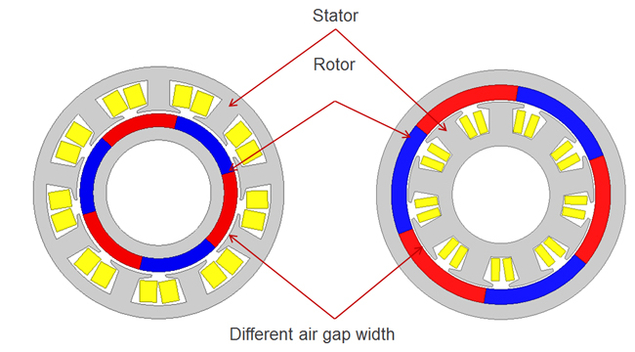
\includegraphics[width=11cm, height= 6cm]{images/Abbildung1.jpg}
        \caption{Innenläufer links – Au{\ss}enläufer rechts 
        \cite{cdyn:BLDC}}
        \label{Innen/Aussenlaeufer}
        \end{center}
\end{figure}

\subsection{Kommutierung}
Die typischste Art, um einen BLDC anzusteuern ist die Kommutierung. Bei dieser Art wird jede Spule abwechselnd ein- und ausgeschaltet, während zwei Spulen aktiv sind, ist eine Spule inaktiv. So kann auch mit Gleichspannung ein Drehfeld erzeugt werden. 
\begin{figure}[h]
    \begin{center}
        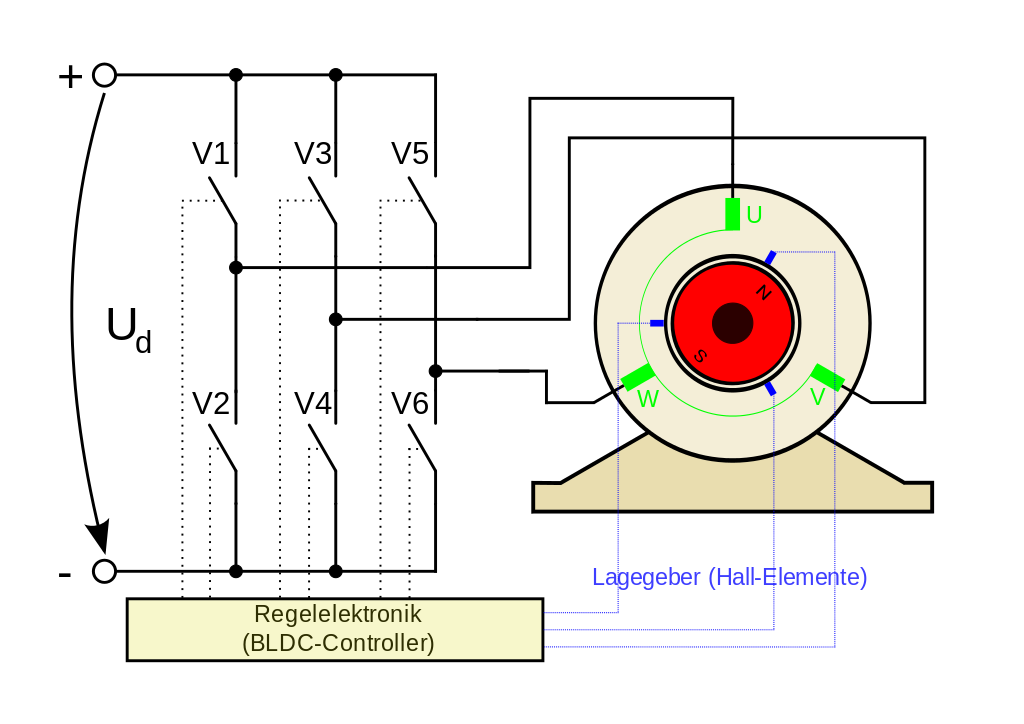
\includegraphics[width=15.35cm, height= 10.85cm]{images/Abbildung 2.png}
        \caption{Dreiphasen Brückenschaltung am BLDC Motor 
        \cite{wiki:BLDC}}
        \label{BrückenschaltungBLDC}
        \end{center}
\end{figure}
Wie in Abbildung 2 werden zum Ein- und Ausschalten drei Halbbrücken verwendet. Als Schalter werden Metal-Oxide Semiconductor Field-Effect Transistor (MOSFET’s) oder Isolated Gate Bipolar Transistors (IGBT’s) verwendet. Durch abwechselndes Durchschalten der Transistoren werden jeweils zwei Wicklungen versorgt und somit wird ein Drehfeld erzeugt. 
\cite{wiki:BLDC}
\cite{sflix:Kommutierung}
\subsubsection{Sensorgesteuerte Kommutierung}
Bei der sensorgesteuerten Kommutierung wird die Rotorposition durch Sensoren erfasst. Sensoren, die verwendet werden können, sind beispielsweise Hall-Sensoren. Diese erkennen die aktuelle Rotorposition durch das Erfassen des magnetischen Flusses. Au{\ss}erdem können optische Sensoren verwendet werden, die am Stator angebracht sind und somit die Position des Rotors erkennen.  Durch die Informationen, die durch das Auslesen dieser Sensoren bereitstehen, kann die Steuerelektronik richtig gesteuert werden, zusätzlich ist es möglich mit solchen Sensoren die Drehzahl zu ermitteln. 
\cite{wiki:BLDC}
\cite{sflix:Kommutierung}
\clearpage
\subsubsection{Sensorlose Kommutierung}
Wenn keine Sensoren verwendet werden, dann handelt es sich um eine sensorlose Kommutierung. Die Spulen werden durch das Erfassen von elektrischen Grö{\ss}en ein- und ausgeschaltet. Diese elektrischen Grö{\ss}en sind beispielsweise Motorstrom- oder Spannung. Aufgrund dieser Grö{\ss}en wird auf die aktuelle Geschwindigkeit des Motors geschlossen und der Kommutierungsblock richtig geschalten. Ein Problem der sensorlosen Kommutierung ist, dass ein Minimum an Drehzahl erreicht werden muss, um eine Gegenspannung im Rotor messen zu können. Diese Art der Kommutierung hat zur Folge, dass beim Anlauf der Maschine blind geschaltet werden muss. 
\cite{wiki:BLDC}
\cite{SPSM:SLKomm}
\subsection{Einsatzbereiche von bürstenlosen Gleichstrommotoren}
BLDC-Motoren haben unzählige Einsatzbereiche einige Beispiele sind: \cite{wiki:BLDC}
\begin{itemize}
    \item Festplatten für PCs und andere Laufwerke, wie DVD oder Blu-Ray \cite{ASPINA:BLDC}
    \begin{itemize}
        \item Diese Motoren werden hier aufgrund ihrer hohen Präzision verwendet. \cite{ASPINA:BLDC}
\end{itemize}
\end{itemize}
\begin{itemize}
    \item E-Mobility \cite{wiki:BLDC}
    \begin{itemize}
        \item Autohersteller nutzen diese Motoren, da sie ohne gro{\ss}en Aufwand mit einem Akku betrieben werden können. 
         Und oft sehr leicht sind. \cite{wiki:BLDC}
        \item Aus diesem Grund werden solche Motoren in der Emily verwendet. 
\end{itemize}
\end{itemize}
\begin{itemize}
    \item Werkzeuge mit Akku \cite{wiki:BLDC}
    \begin{itemize}
        \item Werkzeughersteller tendieren zu BLDC-Motoren, da diese weniger Wartungen als Motoren mit Bürsten benötigen. \cite{wiki:BLDC}
\end{itemize}
\end{itemize}



\section{SONCEBOZ BLDC-Motor (CPM90 5934)}
Der SONCEBOZ BLDC-Motor CPM90 ist ein kleiner BLDC-Motor, der mit maximal 48V versorgt wird, er kann auch mit niedrigeren Spannungsniveaus betrieben werden. Deshalb ist er passend als Testmaschine für den Motorprüfstand. Au{\ss}erdem hat dieses Modell eine integrierte CAN-Bus Ansteuerung, was die Gestaltung der Ansteuerung um vieles leichter macht. \cite{SONCEBOZ}
Dieser BLDC-Motor ist auf der Testbank mechanisch verbaut und für ihn muss eine Software geschrieben werden. 


\begin{figure}[h]
    \begin{center}
        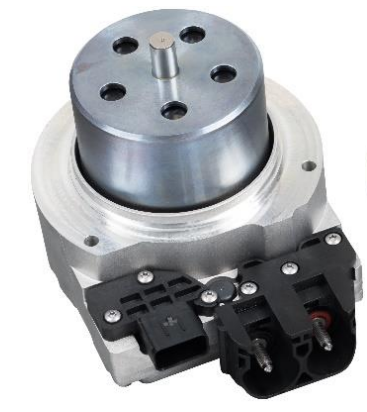
\includegraphics[width=6.68cm, height= 7.5cm]{images/Abbildung 3.png}
        \caption{SONCEBOZ BLDC-Motor CPM90 5934 \cite{SONCEBOZ}}
        \label{SONCEBOZ BLDC}
        \end{center}
\end{figure}
\clearpage
\subsection{Technische Daten}

\begin{table}[ht]
    \centering
    \begin{tabular}{|l | r|} 
        \hline
        Leistung & 5,4kW\\
        \hline
        Drehmoment & 14,2Nm\\
        \hline
        Drehzahl & 600 min$^-$$^1$ \\
        \hline
        Kommunikation & CAN\\
        \hline
        Gewicht & 4,1kg\\
        \hline
        Dimensionen & \emptyset 88,57 x 2.62mm\\
        \hline
        Versorgungsspannung & 48VDC\\
        \hline
    \end{tabular}

    
    \caption{Technische Daten des SONCEBOZ BLDC-Motors \cite{SONCEBOZ}}
    \label{table::tDaten}
\end{table}

\subsection{Funktionsdiagramm und PIN-Belegung}
\begin{figure}[h]
    \begin{center}
        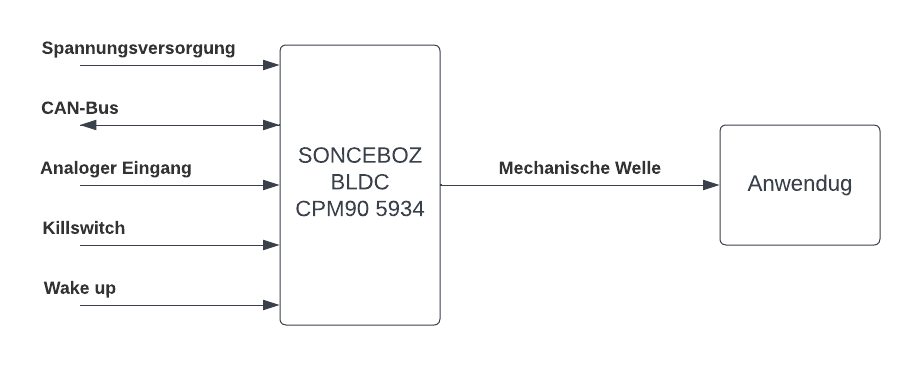
\includegraphics[width=14.61cm, height= 5.79cm]{images/Abbildung 4.png}
        \caption{Funktionsdiagramm des SONCEBOZ BLDC-Motors \cite{SONCEBOZ}}
        \label{Fdiagramm SONCEBOZ BLDC}
        \end{center}
\end{figure}
\clearpage

\begin{table}[ht]
    \begin{center}
    \begin{tabular}{|c | l | l|} 
        \hline
        Pin Nummer & Zuordnung & Kommentar\\
        \hline
        1 & CAN\_L & CAN Low\\
        \hline
        2 & D\_IO\_1 & nicht benutzt \\
        \hline
        3 & CAN\_H & CAN High\\
        \hline
        4 & DGND & nicht benutzt\\
        \hline
        5 & Wake up & Logik aktivieren\\
        \hline
        6 & 5V\_IO & 5V Versorgung für Kill Switch\\
        \hline
        7 & Killswitch & Power Stage aktivieren\\
        \hline
        8 & 5V\_1 & 5V Versorgung für Analog1\_\\
        \hline 
        9 & AN\_1 & Signal Eingang für Analog\_1\\
        \hline 
        10 & A\_GND\_1 & GROUND für Analog\_1\\ 
        \hline
        11 & 5V\_2 & 5V Versorgung für Analog\_2\\
        \hline 
        12 & AN\_2 & Signal Eingang für Analog\_2\\
        \hline  
        13 & A\_GND\_2 & GROUND für Analog\_2\\
        \hline
        14 & 5V\_3 & 5V Versorgung für Analog\_3\\
        \hline 
        15 & AN\_3 & Signal Eingang für Analog\_3\\
        \hline 
        16 & A\_GND\_3 & GROUND für Analog\_3\\
        \hline
    \end{tabular}

    \label{table::PIN-Belegung}
    
    \caption{PIN-Belegung des SONCEBOZ BLDC-Motor \cite{SONCEBOZ}}
\end{center}
\end{table}

Spannungsversorgung:
\begin{itemize}
    \item Die Hauptspannungsversorgung ist auf dem PIN U$_{bat+}$ und dem PIN U$_{bat-}$ des BLDC-Motors, dieser wird mit einem 24V Netzteil versorgt, bei dem zwei Ausgänge in Serie geschalten wurden.  \cite{SONCEBOZ}
\end{itemize}

CAN-Bus:
\begin{itemize}
    \item Der CAN-BUS wird bei den beiden PINs CAN\_L und CAN\_H angeschlossen und dann mit der SPS verbunden, worüber der BLDC-Motor gesteuert wird und verschiedene Informationen vom Motor zur SPS geschickt werden. \cite{SONCEBOZ}
\end{itemize}

Analoge Eingänge:
\begin{itemize}
    \item 
    Die PINs AN\_1, AN\_2 und AN\_3 werden mit maximal 5V versorgt und auf PIN A\_GND\_1, 2 oder 3 auf Masse gelegt. 
    Diese Analogen Signal-Eingänge werden an den Ausgang von externen Sensoren geschlossen, um den Mikrocontroller diese Signale zu senden, 
    dieser wandelt diese Signale um und regelt damit den Motor, falls eine Regelung implementiert wurde, oder gibt die Signale über die CAN-Schnittstelle aus. \cite{SONCEBOZ}
\end{itemize}

Analoge Ausgänge:
\begin{itemize}
    \item Die PINs 5V\_1, 5V\_2 und 5V\_3 werden verwendet, um externe Sensoren zu versorgen. Diese werden auf den jeweiligen PIN A\_GND\_1, 2 oder 3 auf Masse gelegt. In dem Blockschaltbild der Platine ist ersichtlich, dass diese Ausgänge durch die Hauptspannungsversorgung gespeist werden. \cite{SONCEBOZ}
\end{itemize}

Killswitch:
\begin{itemize}
    \item Dieser Schalter hat die Funktion den Motor komplett von der Spannung zu nehmen, er dient also als NOT-Halt. Er ist auf dem PIN 5V\_IO mit 5V versorgt und auf dem PIN Killswitch wird er ausgelöst und somit wird der Motor zum Stillstand gebracht. \cite{SONCEBOZ}
\end{itemize}

Wake up:
\begin{itemize}
    \item Dieser Schalter wird benutzt um die gesamte Spannungsversorgung ein- bzw. auszuschalten. Also dient er unter anderem als NOT-Aus. Das Öffnen dieses Schalters hat jedoch zur Folge, dass auch der Mikrocontroller spannungsfrei wird und somit keine RAM-Erinnerung erhalten bleibt.  \cite{SONCEBOZ}
\end{itemize}

\clearpage
\subsection{Blockschaltbild und Bauteilbeschreibung}

\begin{figure}[h]
        \begin{center}
            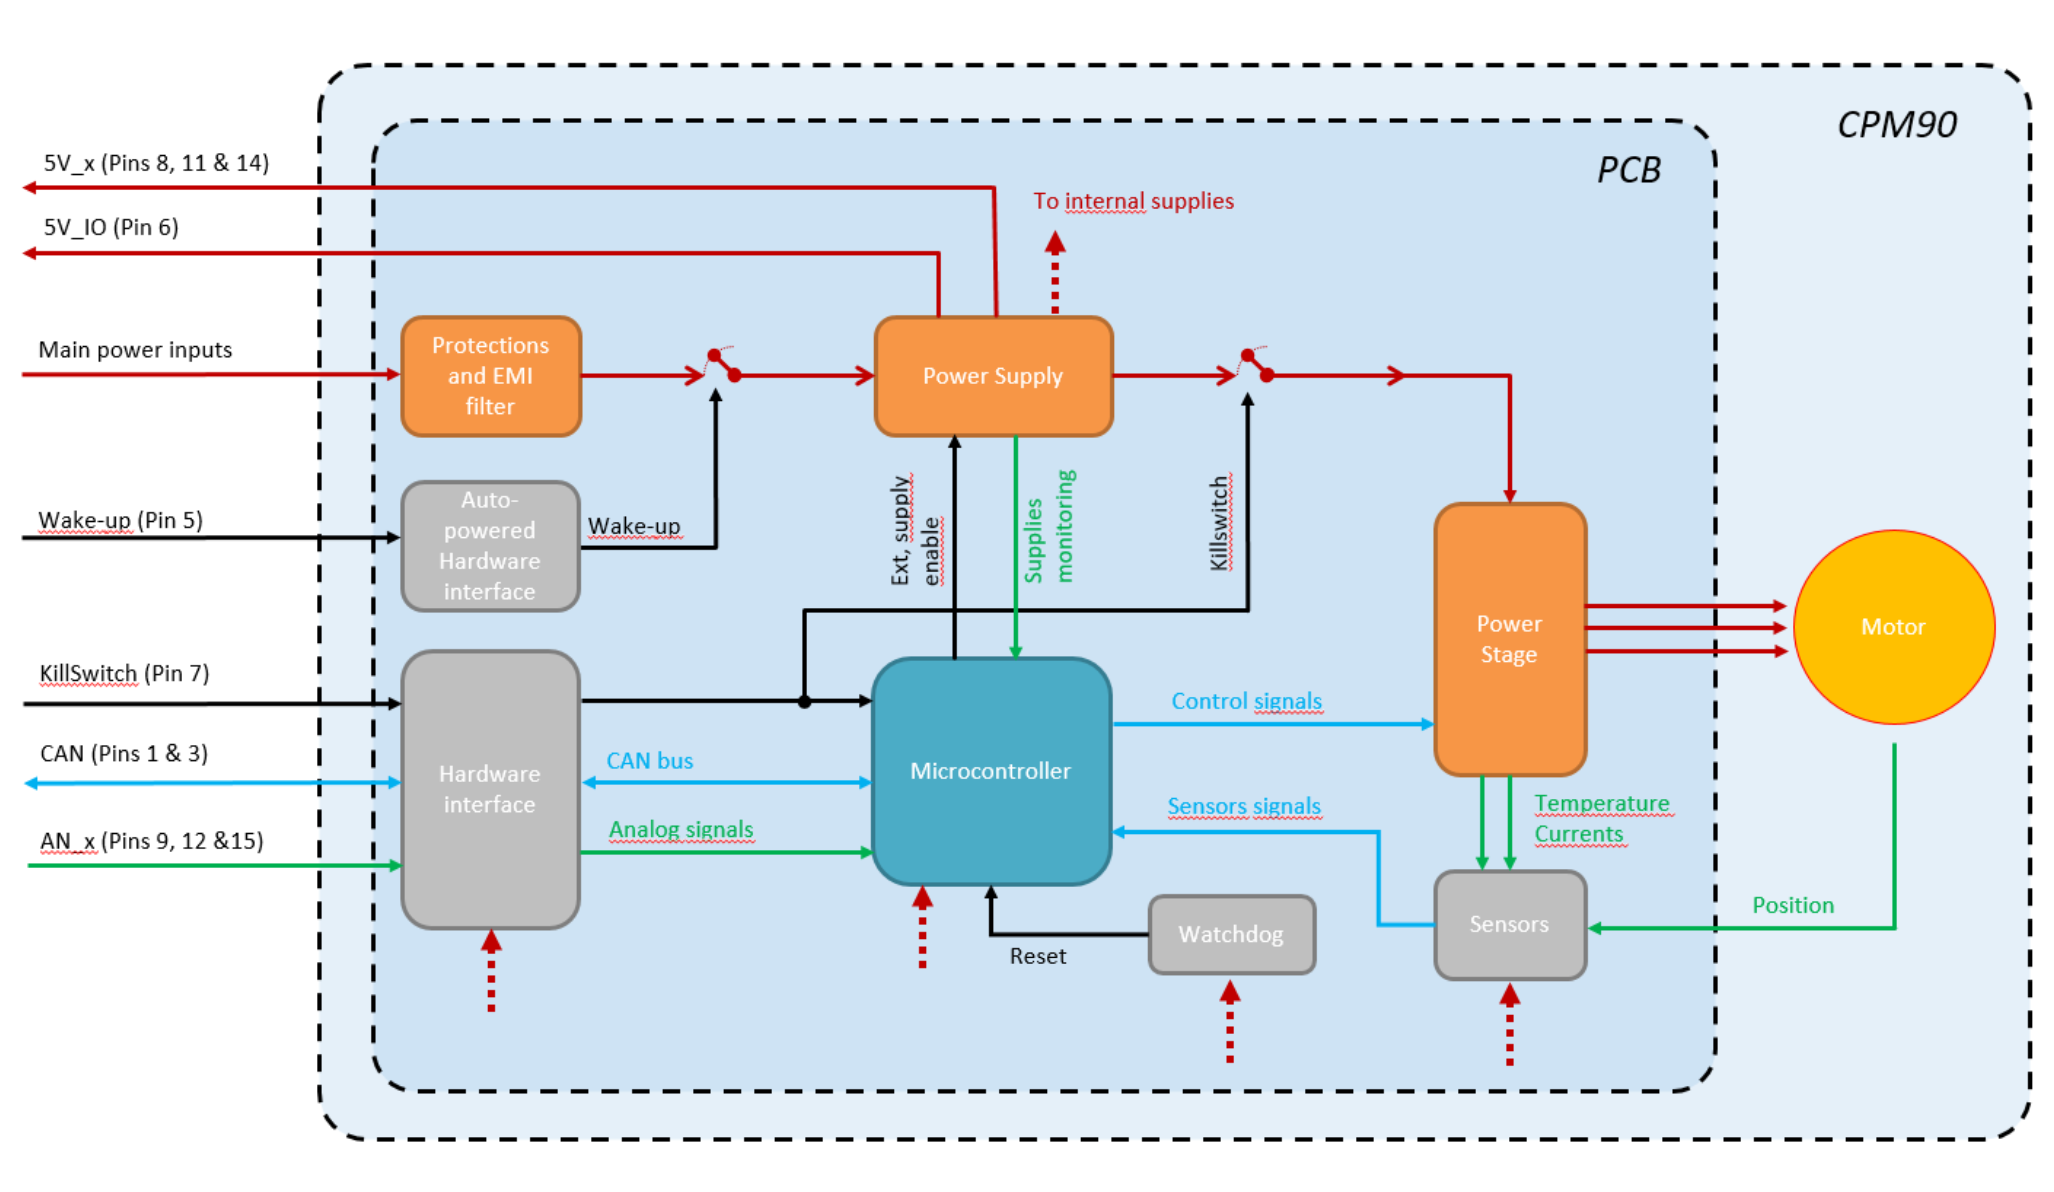
\includegraphics[width=15.76cm, height= 9.15cm]{images/Abbildung 5.png}
            \caption{Blockschaltbild der Elektronik des SONCEBOZ BLDC-Motor \cite{SONCEBOZ}}
            \label{Blockschaltbild BLDC}
            \end{center}
    \end{figure}

Das Blockschaltbild in Abbildung 5 gibt die verschiedenen Komponenten und Signalpfade auf dem Printed Curcuit Board (PCB) des SONCEBOZ BLDC-Motormodells CPM90 an. \\

Die roten Pfeile symbolisieren die verschiedenen Spannungsversorgungen, die ersten zwei sind die Versorgungen für externe Sensoren, der dritte Pfeil von oben ist die Hauptspannungsversorgung für den Motor. 
Die schwarzen Pfeile geben den Weg von Wake up und Killswitch an und die jeweiligen Schalter. 
Die blauen Pfeile zeigen die Wege der CAN-Signale an. Diese werden im Mikrocontroller verarbeitet und steuern den Motor. Au{\ss}erdem geben die Sensoren, die die Position des Motors erfassen ein CAN-Signal an den Mikrocontroller weiter das ausgelesen werden kann. Mit diesem Signal ist es beispielsweise möglich die Drehzahl ausgeben zu lassen.
Die grünen Pfeile sind analoge Ausgänge der externen Sensoren, die im Mikrocontroller verarbeitet werden. \cite{SONCEBOZ}\\


EMV Filter:
\begin{itemize}
    \item Der EMV-Filter wird verwendet, um Störungen von nahegelegenen Kapazitäten und Induktivitäten zu unterdrücken, au{\ss}erdem hilft er dabei andere Geräte nicht zu beeinflussen. \cite{SONCEBOZ}
\end{itemize}

Spannungsversorgung:
\begin{itemize}
    \item Von diesem Punkt werden alle Geräte auf der Platine versorgt. \cite{SONCEBOZ}
\end{itemize}

Leistungsstufe:
\begin{itemize}
    \item Die Leistungsstufe erhält Signale von dem Mikrocontroller und steuert passierend auf diesen den Motor. \cite{SONCEBOZ}
\end{itemize}

Selbstversorgte-Hardware-Schnittstelle:
\begin{itemize}
    \item Diese Schnittstelle ist vorhanden um den Wake up Schalter zu steuern. \cite{SONCEBOZ}
\end{itemize}

Hardware-Schnittstelle:
\begin{itemize}
    \item An dieser Schnittstelle werden alle relevanten Dinge für den Mikrocontroller angeschlossen. \cite{SONCEBOZ}
\end{itemize}

\clearpage
Watchdog:
\begin{itemize}
    \item Der Watchdog ist ein digitales System, dass die gesamte Platine überwacht und notfalls die gesamte Spannungsversorgung ausschalten kann, falls es zu schweren Schäden kommen könnte. \cite{SONCEBOZ}
\end{itemize}

Sensoren:
\begin{itemize}
    \item Das sind Sensoren, die extern und intern vorhanden sein können. Interne Sensoren sind beispielsweise solche die die Rotorposition erkennen, um den Motor zu steuern. Externe Sensoren können alle möglichen Funktionen haben und werden wie bereits beschrieben von den analogen Outputs versorgt und deren Ausgang wird bei den analogen Inputs angeschlossen. \cite{SONCEBOZ}
\end{itemize}

Mikrocontroller:
\begin{itemize}
    \item Dieser steuert alle Vorgänge auf der Platine. Er steuert die Schaltvorgänge die den Motor zum Laufen bringen. Au{\ss}erdem liest er Sensoren aus und wandelt analoge Signale in digitale um. \cite{SONCEBOZ}
\end{itemize}



\section{CAN-Bus}
CAN steht für Controller Area Network und gehört zu den Feldbussystemen. Dieses Feldbussystem findet zahlreiche Anwendungsmöglichkeiten unter anderem in der Automobilindustrie, Automatisierungstechnik und in vielen weiteren Bereichen. In dieser Arbeit wurde der Feldbus verwendet, um mit dem BLDC-Motor zu kommunizieren. 

\subsection{Funktionsweise}
Bei CAN-Bus Systemen sind mehrere gleichrangige Steuerelemente miteinander verbunden, dieses Prinzip hei{\ss}t „Multi-Master-Prinzip“. Um Kollisionen zu lösen, wird das CSMA/CR-Verfahren eingesetzt, dazu muss es verschieden hochrangige Zustände geben. Bei diesem System hat die logische 0 eine höhere Priorität und wird bei einer Kollision somit übertragen. Wenn der CAN-Bus mit Kupferleitungen arbeitet, werden zwei Adern miteinander verdrillt, diese fungieren als CAN HIGH (CAN\_H) und CAN LOW (CAN\_L) und haben verschieden hohe Spannungspotenziale (z.B.: CAN\_H: 5V und CAN\_L: 3V). Diesen Vorgang wird NRZ-Bitcodierung (Non Return to Zero) genannt. Somit werden die Eigenschaften der symmetrischen Signalübertragung genutzt, um Störungen minimal zu halten bzw. ganz auszulöschen. Je höher die Übertragungsrate sein soll, desto niedriger muss die Spannungsdifferenz zwischen CAN HIGH und CAN LOW sein und desto niedriger ist die maximale Reichweite. 

\clearpage

\subsubsection{Multimaster Prinzip}
Bei dem Multimaster Prinzip gibt es mehrere Master, die über ein Gateway miteinander kommunizieren können. \\
Das kann so wie in Abbildung 6 aussehen. \\

\begin{figure}[h]
    \begin{center}
        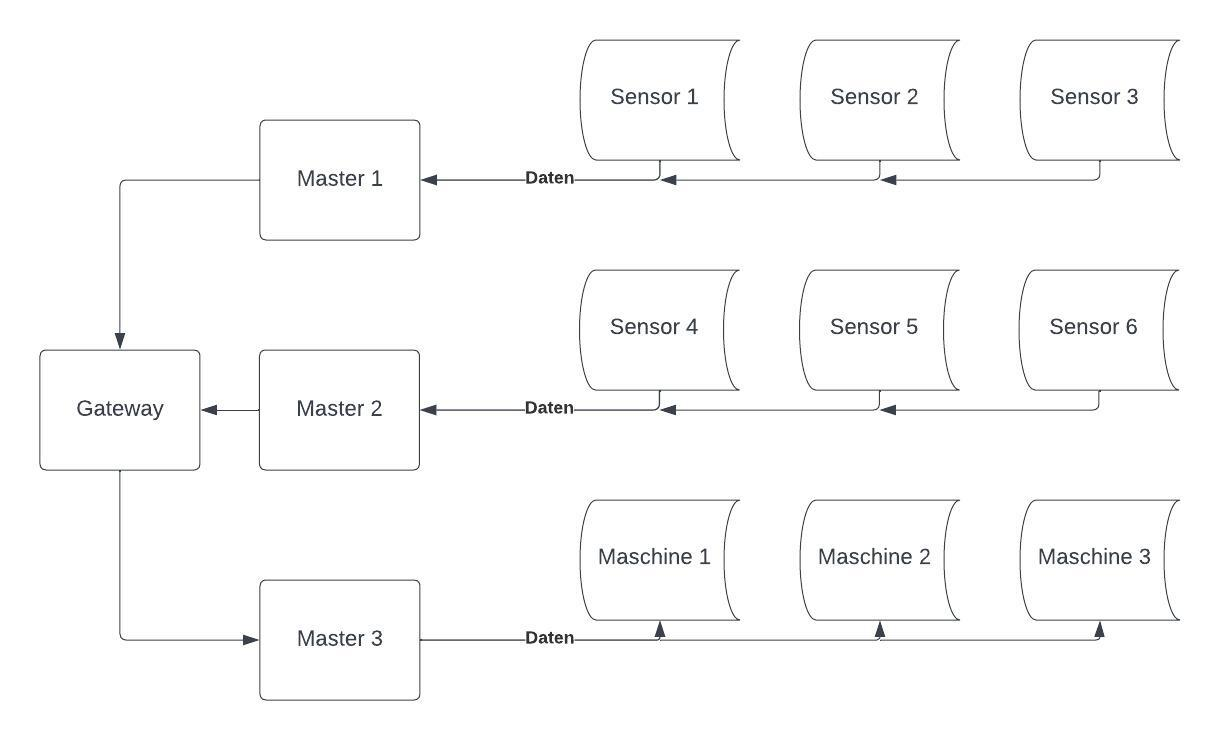
\includegraphics[width=13.98cm, height= 8.48cm]{images/Abbildung 6.jpeg}
        \caption{Multimaster Prinzip}
        \label{MMaster}
        \end{center}
\end{figure}

In diesem Beispiel senden Master eins und zwei Daten, die sie von den Sensoren erhalten, Master drei verarbeitet diese Daten und steuert damit seine Maschinen. Bei diesem Prinzip ist es möglich das zwei Master gleichzeitig senden und es somit zu einer Kollision kommt. Welcher von beiden seine Nachricht durchführen darf, wird nach dem CSMA/CR Protokoll entschieden. 

\clearpage
\subsubsection{CSMA/CR}
Carrier Sense Multiple Access / Collision Resolution funktioniert aufgrund von Bitarbitrierung. Ein Bitarbitrierer ist eine Schaltung, die möglichst schnell entscheiden kann, welches von beiden gesendeten Signalen eine höhere Priorität hat. Eine Kollision wird also erkannt, und dann anders wie bei CSMA/CA nicht abgewartet, sondern entschieden welches von den beiden Signalen den freien Sendeplatz bekommt. In Abbildung 7 ist dieser Verlauf verbildlicht. \\

\begin{figure}[h]
    \begin{center}
        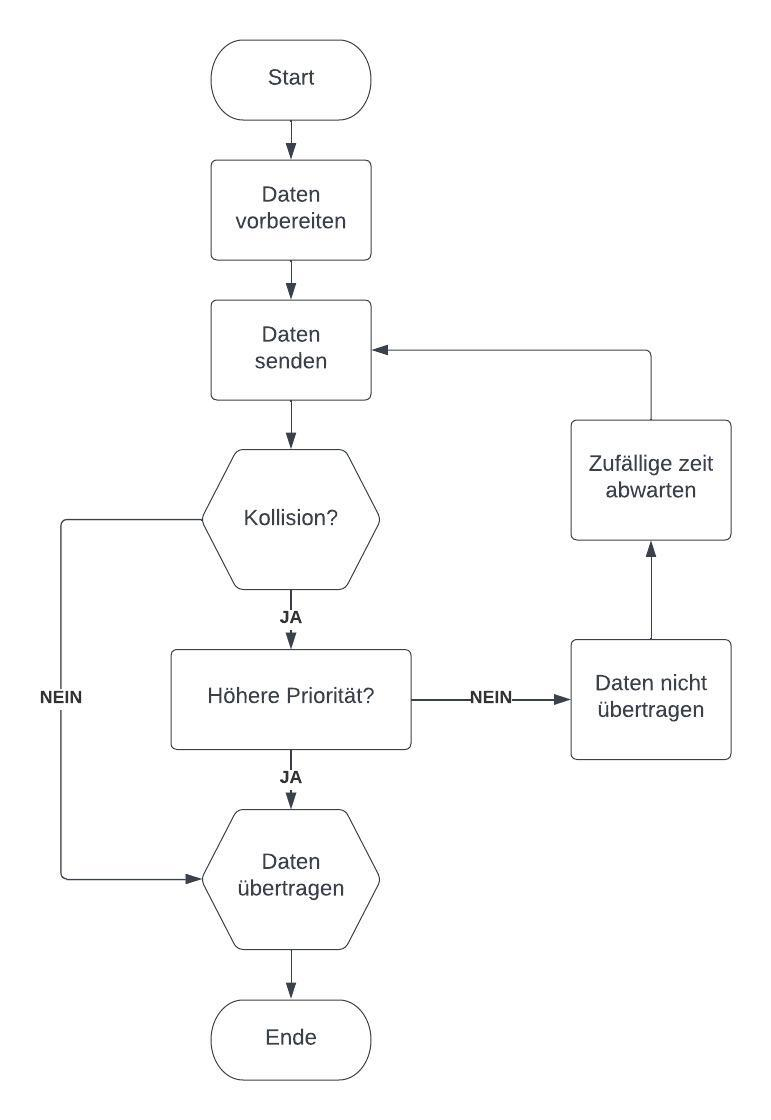
\includegraphics[width=12.24cm, height= 17.78cm]{images/Abbildung 7.jpeg}
        \caption{CSMA/CR Flussdiagramm}
        \label{CSMA/CR}
        \end{center}
\end{figure}

\clearpage

\subsubsection{Non Return to Zero (NRZ-Bitcodierung)}
Die NRZ-Bitcodierung wurde für CAN-Bussysteme gewählt, denn diese Art von Codierung erlaubt hohe Datenraten mit sehr geringen Verlusten. In diesem Fall gibt es keinen Leiter mit einem Null-Potential, ein dominantes Bit wird durch ein hohen Potenzialunterschied und ein rezessives Bit wird durch einen niedrigen Potenzialunterschied dargestellt. In Abbildung 8 ist das an einem Beispiel von Highspeed-CAN verbildlicht. \\

\begin{figure}[h]
    \begin{center}
        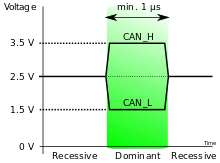
\includegraphics[width=8.66cm, height=6.39cm]{images/Abbildung 8.png}
        \caption{Spannungsdifferenz im Highspeed-CAN}
        \label{Highspeed-CAN}
        \end{center}
\end{figure}
Ein Nachteil dieser Bitcodierung ist, dass der Empfänger die Synchronisation verliert, wenn der Pegel lange unverändert bleibt. Die Lösung zu diesem Problem nennt sich Bitstuffing. Dieser Synchronisierungsmechanismus sendet nach fünf homogenen Bits ein komplementäres Bit, dass dem Empfänger den Takt vorgibt. \\

\subsection{Topologie}
Der Aufbau von CAN-Bus Systemen ist meist einer Linie entlang strukturiert, es gibt auch sternförmige Topologien, diese haben im Vergleich jedoch Nachteile. Da sternförmige Aufbauten meist über einen Hauptrechner laufen, kommt es beim Ausfall von diesem zu einem kompletten Ausfall des Systems. Bei der häufigsten Art kann es nur bei einem Ausfall der Adern zu einem Komplettausfall kommen. \\

\begin{figure}[h]
    \begin{center}
        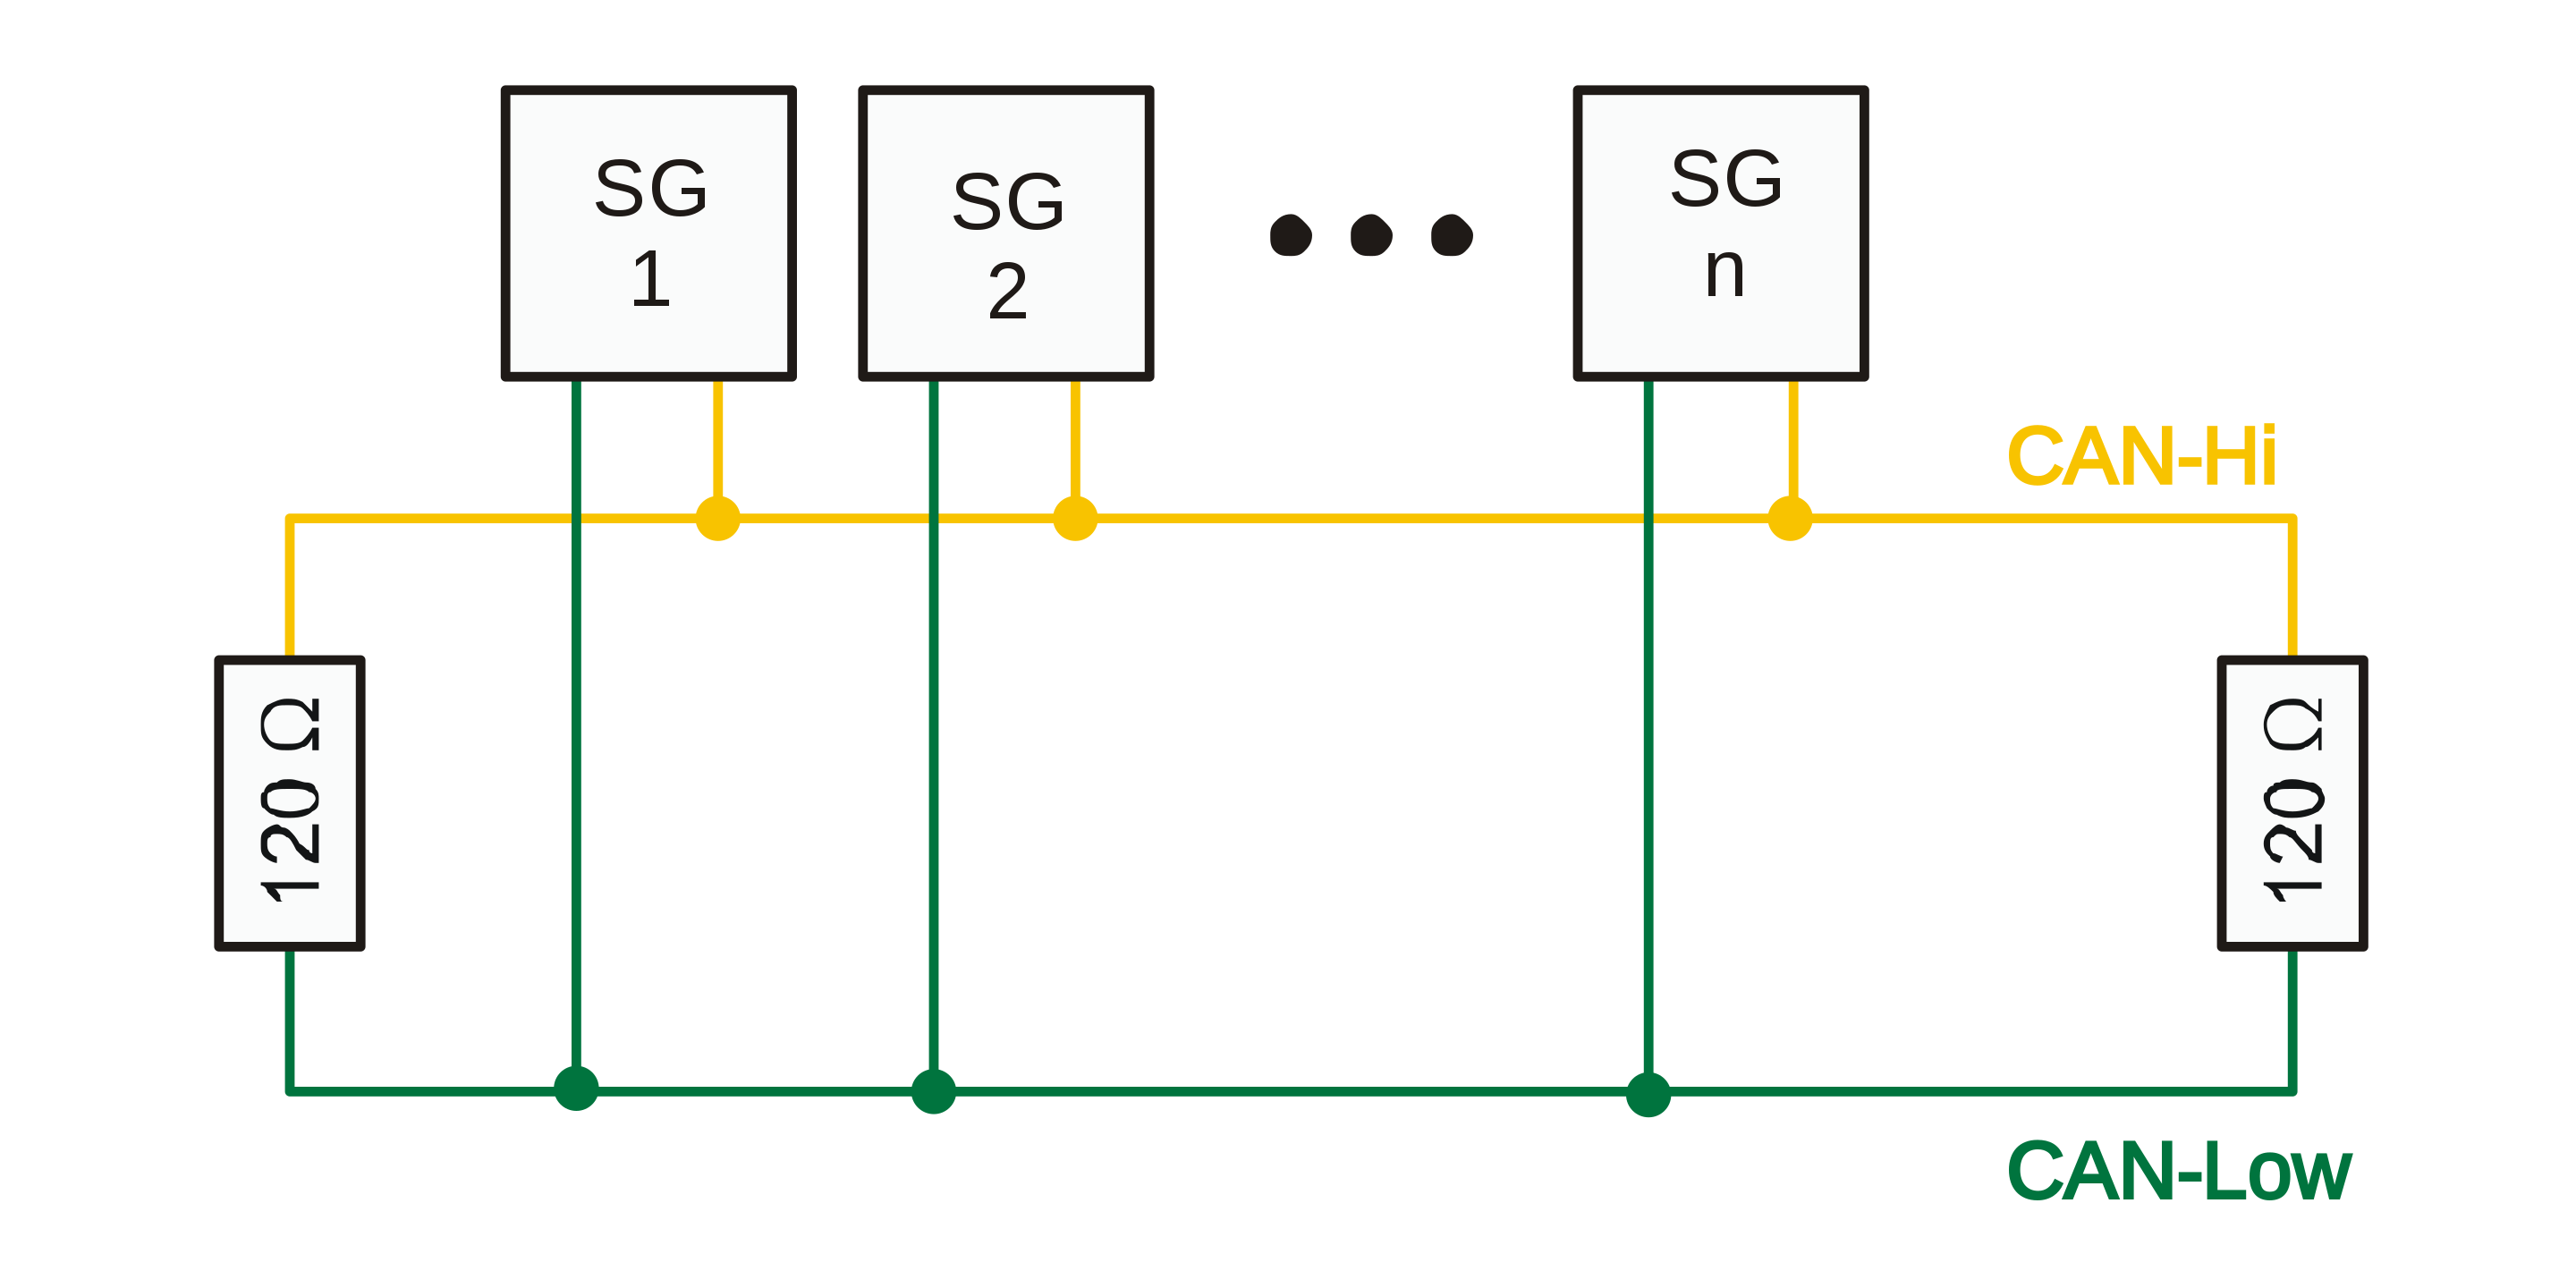
\includegraphics[width=10.08cm, height=5.04cm]{images/Abbildung 9.png}
        \caption{CAN-Bus in Linientopologie}
        \label{Linientopologie}
        \end{center}
\end{figure}
Die Abschlusswiderstände von 120 Ohm sind vorhanden, um Reflexionen zu vermeiden. Eine Reflexion von Wellen ist die Überlagerung von einer zurücklaufenden Welle und einer vorlaufenden Welle, dass bildet eine stehende Welle auf der Leitung und beeinflusst das Signal. 

\clearpage

\subsection{Anwendungsbereiche}


\printLiteratur     % Literatur
\printAbbildungen   % Abbildungsverzeichnis
\printTabellen      % Tabellenverzeichnis
\printAkronyme      % Abkürzungsverzeichnis
\printFullChangelog % Vollständiger Änderungsverlauf

\end{document}